
\chapter[Domaine métier]{Domaine métier}
Dans le restaurant Crazy Wolf et dans la restauration en général, les employés sont susceptibles de ne pas travailler tous les jours ou de ne pas travailler toute la journée mais seulement certains "services".

Un service est une tranche horaire qui correspond aux heures pendand lesquelles le restaurant offre un service de restauration. Dans le cas concret du Crazy Wolf, il y a deux services: midi et soir. Qui englobent les heures de travaille de 9h00 à 15h00 et de 17h00 à 23h00 respectivement. Dans ces tranches horaires sont inclus les heures nécéssaires à la disposition du restaurant et d'autres préparations nécéssaires avant l'arrivée de clients.

De plus, dans la restauration et surtout en se qui concerne les serveurs, il est commun d'y trouver trois types d'acteurs avec différents statuts: 
\smallskip
\begin{itemize}
    \item serveur$\cdot$euses
    \item manager 
    \item patrons
\end{itemize}
\smallskip
La gestion, visualisation et organisation des services parmis ces trois acteurs est un élément vital pour un restaurant.

\section[Analyse]{Analyse}
D'après mon observation, la plannification de l'horaire de travail des serveurs à un moment donné n'est pas invariante par rapport au temps. En d'autres termes, entre le moment où l'attribution de services aux serveurs est faite et le moment où un serveur y travaille effectivemnt il peut y avoir de grandes variations. J'ai constaté essentiellement trois facteurs susceptibles de perturber la plannification initial:
\smallskip
\begin{itemize}
    \item le désistement d'un$\cdot$ serveur$\cdot$euses
    \item les échanges
    \item la demande de renfort de la part du manager ou d'un patron.
\end{itemize}
\smallskip
Le premier peut être dû à diverses raisons: maladie, imprévu... De plus comme dans le Crazy Wolf, la majorité des serveur$\cdot$euses sont étudiant$\cdot$es les révisions, examens et autres sont aussi souvent cause de désistement.

Le deuxième est le fruit d'un mutuel accord entre deux serveurs pour échanger leurs services.

Le troisième est le fruit de l'analyse d'afluence des clients de la manager en accord avec les patrons. En effet, s'ils constatent que tout d'un coup l'afluence des clients augmente le jeudi soir et qu'il y a de fortes chances pour que ce soit aussi le cas le vendredi soir, il sera nécessaire de demander un ou des serveurs supplémentaires. 

Les raisons de cette afluence augmentée peuvent être très diverses. Les conditions météo par exemple. Plus de gens vont au Crazy Wolf quand il pleut, ou en hiver. Ou encore des manifestations comme carnaval ou le marathon.

Dans le jargon propre au Crazy Wolf, ces serveurs supplémentaires sont appelés "doubleurs".

Ainsi, la gestion des horaires est dynamique et non statique.

\section[Problématique]{Définition de la problématique}
Actuellement, le Crazy Wolf utilise un groupe, contenant tout le personel, d'une messagerie instantannée pour communiquer. Dans ce groupe sont traîtés toute sorte d'aspects. Depuis des félicitations d'anniversaires, jusqu'à l'envoi des horaires mensuels sous forme pdf en passant par des discutions d'échanges, de remplacements, de renforts ou encore sur des discutions relatives au normes sanitaires dûes à la pandemie du COVID-19. 

Ainsi, lorsque la manager demande un renfort pour dans deux semaines et que personne ne se porte volontaire immédiatement, il y a de grandes chance que le message soit répété plusieurs fois.

Il est donc nécéssaire de disposer d'une plateforme dynamique, standardisée, centralisée et intuitive dédiée exclusivement à la gestion des horaires. 

Cette platteforme doit être accesible en tout temps depuis internet. Une application fonctionnant sur les deux principaux systèmes d'exploitations mobiles répond bien à ce besoin.

En somme, cette application doit fournir les fonctionalités suivantes:

\subsection*{Login}
L'application doit permetre aux utilisateurs de s'authentifier pour accèder à l'ensemble des fonctionnalités.

\begin{figure}[!h]
    \begin{center}
        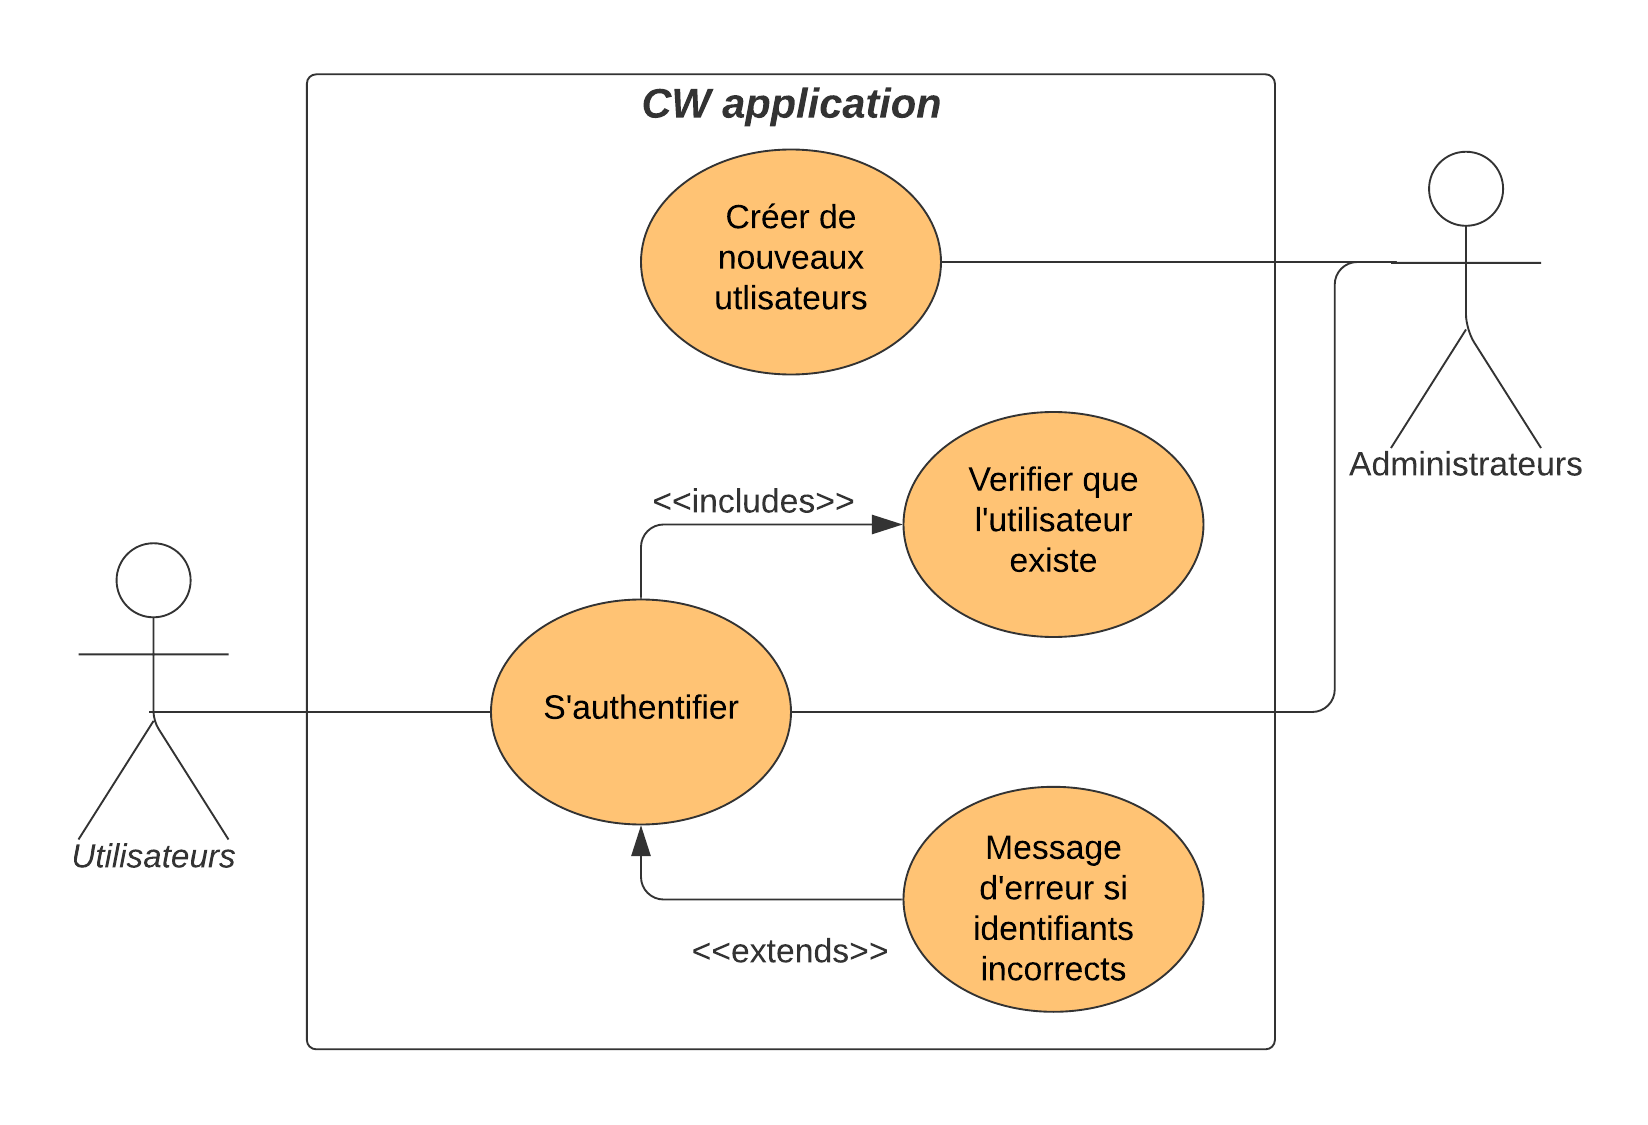
\includegraphics[width= 0.8\textwidth]{uses cases/logginUC.png}
    \end{center}
    \caption{use case: login}
\end{figure}

Pour que l'authentification soit validée, l'utilisateur doit posséder des identifiants qu'un administrateur à créer précédement. Attention, administrateur doit aussi s'authentifier pour pouvoir créer de nouveaux utilisateurs.

De plus, les utilisateurs doivent être informés si leur saisie est incorrecte.

\subsection*{Visualiser les services}
L'application doit permettre à tous les utilisateur de consulter rapidement et facilement les services dans lesquels ils travaillent. De plus, il doivent également pouvoir voir les services dans lesquels les autres utilisateurs travaillent. En effet, il n'y a là aucune information confidentielle.

\begin{figure}[!h]
    \begin{center}
        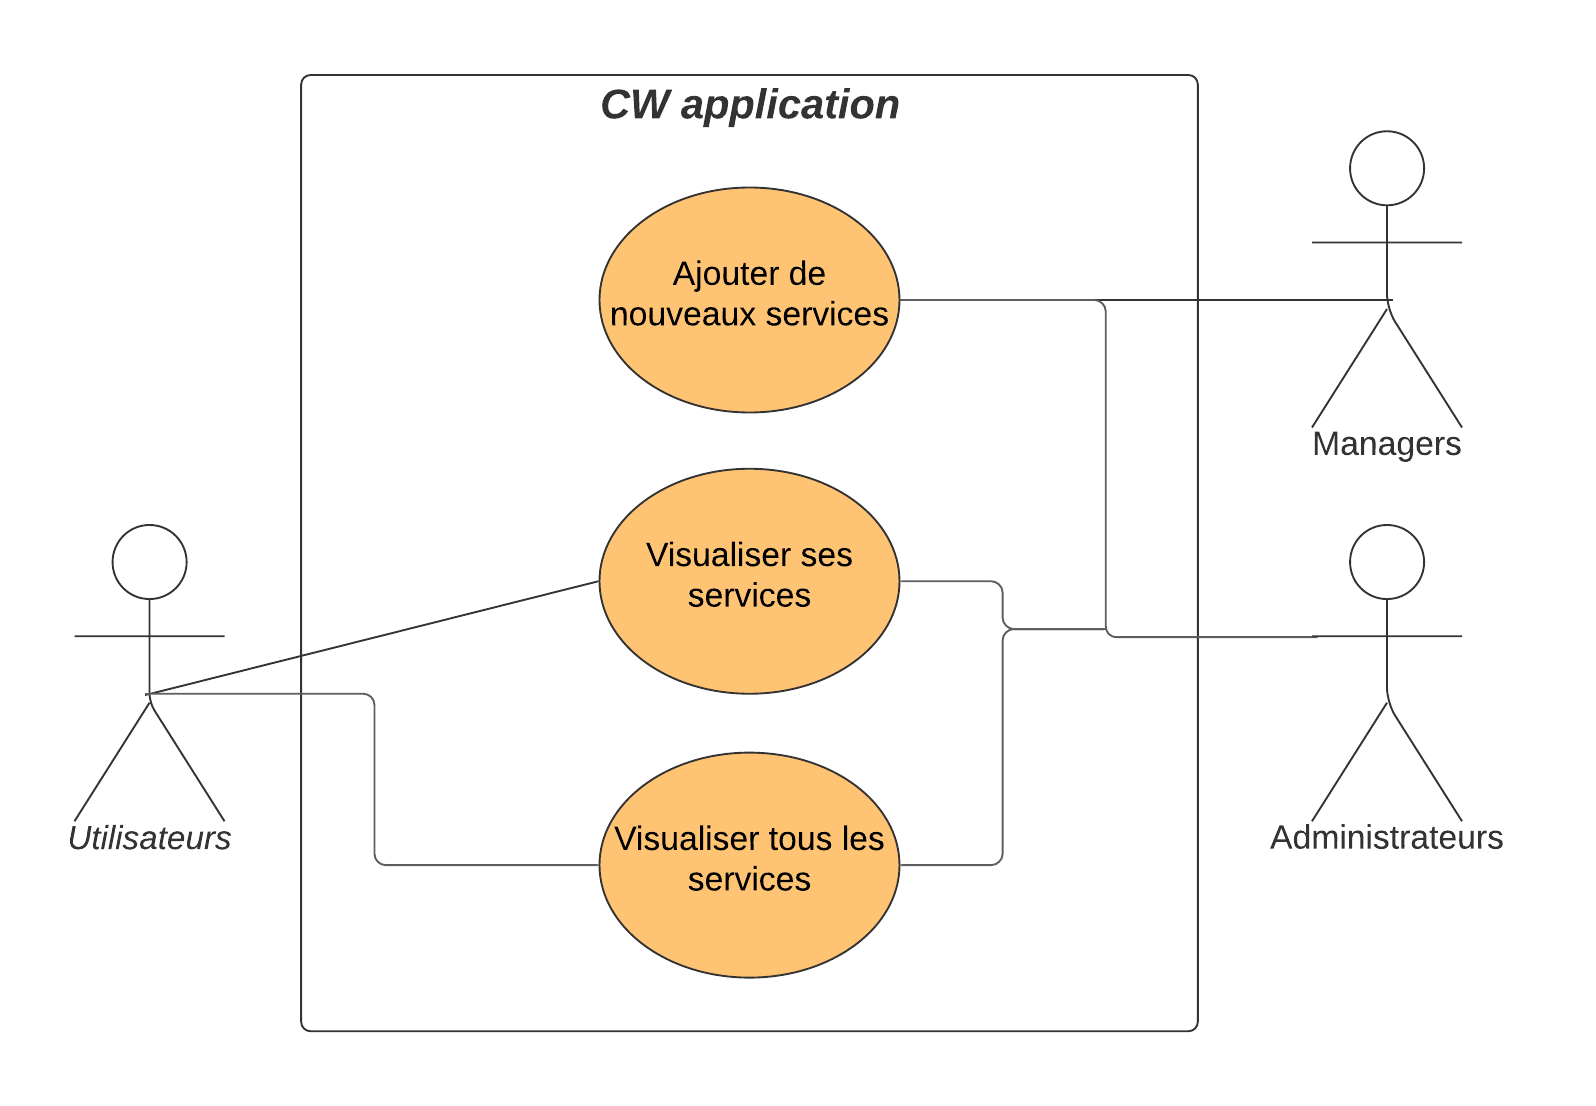
\includegraphics[width= 0.8\textwidth]{uses cases/visualiser services.png}
    \end{center}
    \caption{use case: visualisation des services}
\end{figure}